%======================================================================
\NEWSEC
%======================================================================

\subsection{Particles}
% \subsection{Classes for representing particle data}

\begin{frame}[fragile,label=ss-particles] 
\secframetitle{Classes for representing particle data}
\begin{center}
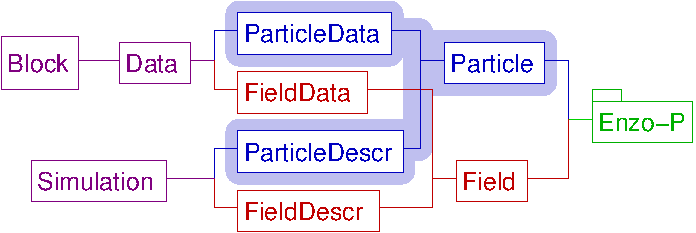
\includegraphics[width=2in]{data-classes-particle.pdf}
\end{center}

\begin{itemize}
\item \greencode{ParticleData}
\begin{itemize}
\item represents state-independent (intrinsic) data
\item associated with \greencode{Block}s (one object per mesh node)
\item stores arrays of particle data
\end{itemize}
\item \greencode{ParticleDescr}
\begin{itemize}
\item represents state-dependent (extrinsic) data
\item associated with \greencode{Simulation} objects (one per process)
\item describes how to interpret particle data (types, attributes, etc.)
\end{itemize}
\item \greencode{Particle}
\begin{itemize}
\item applications access particle data via \greencode{Particle} objects
\end{itemize}
\end{itemize}
\end{frame}

%----------------------------------------------------------------------

\begin{frame}[fragile,label=ss-particles] 
\secframetitle{How \code{Particle} objects store particle data}
\begin{minipage}{1.8in}
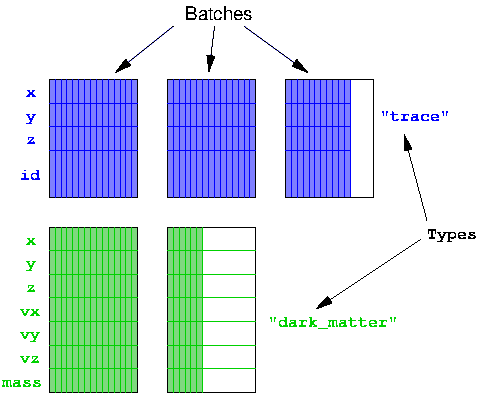
\includegraphics[width=2.0in]{particles-design.pdf} \ \\
\end{minipage} \ 
\begin{minipage}{2.5in}
\begin{itemize}
\item multiple particle \textit{types}
\item particles allocated in \textit{batches}
\begin{itemize}
\item fixed size arrays
\item fewer new/delete operations
\item efficient insert/delete operations
\item potentially useful for GPU's
\end{itemize}
\item batches store particle \textit{attributes}
\begin{itemize}
\item (position, velocity, mass, etc.)
\item 8,16,32,64-bit integers
\item 32,64,128-bit floats
\end{itemize}
\end{itemize}
\end{minipage}
\begin{itemize}
\item particle positions may be floating-point or integers
\begin{itemize}
\item floating-point for storing global positions
\item integers for \code{Block}-local coordinates
\begin{itemize}
\item solves reduced precision issue for deep hierarchies
\item less memory required for given accuracy
\end{itemize}
\end{itemize}
\end{itemize}


\end{frame}

%----------------------------------------------------------------------

\begin{frame}[fragile,label=ss-particles] 
\secframetitle{How particle data is communicated between Blocks}
\begin{itemize}
\item communication is required when particles move outside a Block 
\item this is done using a 4x4x4 array
\begin{itemize}
\item array contains pointers to ParticleData (PD) objects
\item one PD object per neighbor Block
\end{itemize}

\end{itemize}
\begin{minipage}{1.8in}
%\includegraphics<1>[width=2.0in]{particle-refresh-0.pdf}
%\includegraphics<2>[width=2.0in]{particle-refresh-1.pdf}
%\includegraphics<3>[width=2.0in]{particle-refresh-2.pdf}
%\includegraphics<4>[width=2.0in]{particle-refresh-3.pdf}
\includegraphics[width=2.0in]{particle-refresh-4.pdf}
\end{minipage} \ 
\begin{minipage}{2.7in}
\begin{itemize}
\item migrating particles are
\begin{itemize}
\item \code{scatter()}-ed to PD array objects
\item sent to associated neighbors
\item \code{gather()}-ed by neighbors
\end{itemize}
\item one sweep through particles
\item one communication step per neighbor
\item similar for refinement / coarsening
\end{itemize}
\end{minipage}
\end{frame}


